

\begin{table}[htbp]
\centering
\caption{Anti Persona}
\label{tab:Table_persona4}
\small
\begin{tabular}{| m{0.25\textwidth} m{0.65\textwidth}|}
\hline \multicolumn{2}{|c|}{\textbf{Identidade}} \\ \hline
& \\

\begin{center} 
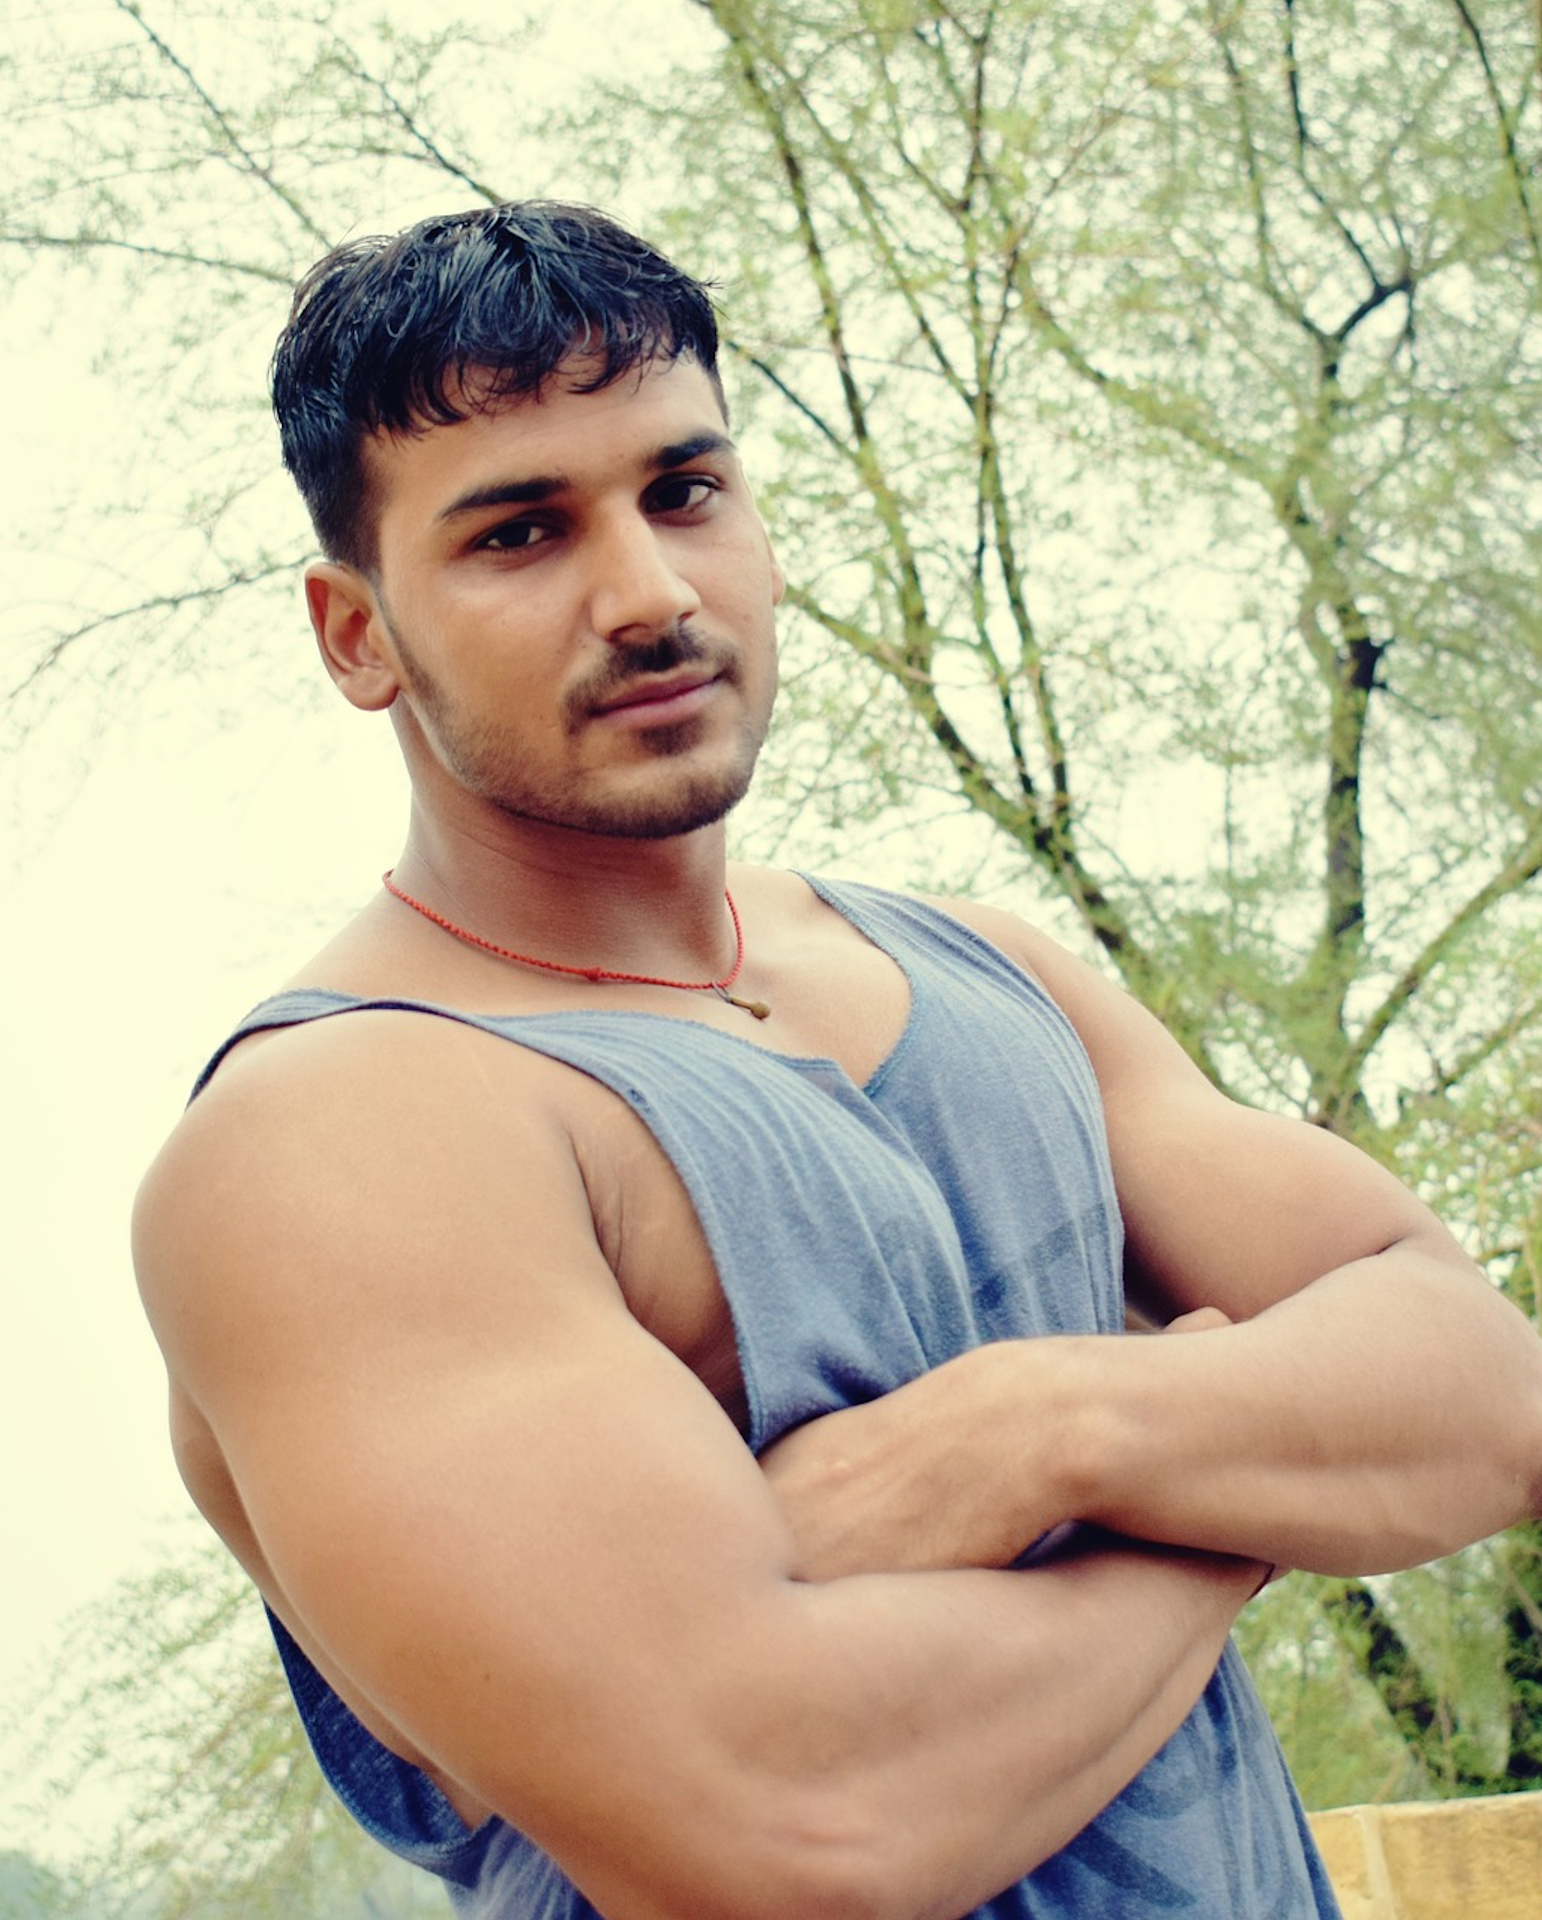
\includegraphics[scale=0.06]{figuras/personas/man-1209494_1920.jpg} 
Fonte: Pixabay\tablefootnote{https://pixabay.com/photos/biceps-aesthetics-body-fitness-2746490/}
\end{center} 

&

\textbf{Nome: }  Rafael Medeiros

\textbf{Idade:} 28 anos

\textbf{Ocupação:} Estudante de Educação Física na UnB, campus Darcy Ribeiro.

\\ \hline


\multicolumn{2}{|c|}{\textbf{Descrição}} \\ \hline
\multicolumn{2}{|p{15cm}|}{
    \begin{tabular}[c]{@{}l@{}}\\
        Não tenho o costume de usar jogos educacionais, devo ter jogado uma vez ou outra, mas\\ não me interessei muito e rapidamente o jogo se tornou monótono pra mim. Gosto mais\\ de jogos esportivos como futebol e basquete. Em relação ao conhecimento\\ acadêmico, me concentro apenas nas disciplinas do meu curso.\\
        \\
        No geral, sou bem competitivo, dou o sangue para \textbf{conquistar} um gol ou fazer um ponto,\\ e fico mais ainda quando se trata de campeonatos, luto pra \textbf{ficar em primeiro}. Em \\jogos digitais eu gosto de ser envolvido com uma \textbf{história} bacana e fico bastante\\ empolgado com \textbf{gráficos} bem realistas e sofisticados. \\
        \\
        Sou mais fã de jogos com trabalho em \textbf{equipe} do que jogos individuais. Gosto tanto\\ atividades competitivas e lúdicas que se desse pra aprender com elas eu com certeza \\trocaria qualquer livro pra \textbf{aprender me divertindo}.\\
        \\
        Como futuro profissional da área de Educação Física meu foco está no estudo de formas\\ de estender o esporte e jogos para públicos com \textbf{necessidades especiais}.\\
        \\
    \end{tabular}
} \\ \hline
\end{tabular}
\end{table}